\documentclass[11pt,a4paper]{article}


\setlength{\parindent}{0pt}

\makeatletter
\renewcommand\section{\@startsection
	{section}{1}{0mm}%			% name, ebene, einzug
	{0pt}%				% vor-abstand
	{24pt}%				% nach-abstand
	{\bfseries\Large}%		% layout
}
\makeatother
\makeatletter
\renewcommand\subsection{\@startsection
	{subsection}{2}{0mm}%			% name, ebene, einzug
	{0pt}%				% vor-abstand
	{12pt}%				% nach-abstand
	{\bfseries\large}%		% layout
}
\makeatother
\makeatletter
\renewcommand\subsubsection{\@startsection
	{subsubsection}{3}{0mm}%			% name, ebene, einzug
	{0pt}%				% vor-abstand
	{6pt}%				% nach-abstand
	{\bfseries}%		% layout
}
\makeatother
\makeatletter
\renewcommand\paragraph{\@startsection
	{paragraph}{4}{0mm}%			% name, ebene, einzug
	{0pt}%				% vor-abstand
	{6pt}%				% nach-abstand
	{\bfseries}%		% layout
}
\makeatother

\usepackage[german]{babel}
%\usepackage{germanb}

%\usepackage{titling}
\usepackage{scrextend}

\usepackage{listings}
\lstset{
	frame=trbl,
	language=SQL,
	breaklines=true}

\usepackage{icomma}

\usepackage{graphicx}
\graphicspath{ {./images/} }

\usepackage{scrlayer-scrpage}
\clearpairofpagestyles
\ofoot{\pagemark}
\ihead{
\includegraphics[height=1cm]{itcLogo}}
%\ohead{\normalfont{\headmark}}
%\automark{section}

\usepackage{tikz}
\usetikzlibrary{er,positioning}

%\usepackage{pgf-umlcd}

\usepackage{svg}
\svgpath{ {./images/} }

\usepackage[left=3.0cm, right=2.5cm, top=3.0cm, bottom=2.5cm, footskip=1.3cm]{geometry}

\usepackage{fontspec}
%\setmainfont{Arial}
\setmainfont{Liberation Sans}

\sloppy

\usepackage{setspace}
\setstretch{1.3}

\usepackage{hyperref}
\hypersetup{
	pdfborder={0 0 0},
	bookmarks=false,
	colorlinks=true,
	linkcolor=[RGB]{0,110,199},
	urlcolor=[RGB]{0,110,199}
}

%[toc, section=section, numberedsection=autolabel]
\usepackage[toc, nonumberlist, acronyms]{glossaries}
\usepackage{glossaries-extra}

\makenoidxglossaries

% !TeX root = Dokumentation.tex

\newglossaryentry{git}{
	name={Git}, 
	description={
		Quelle: \href{https://git-scm.com/book/en/v2F}{https://git-scm.com/book/en/v2}\newline
		Git ist ein Open-Source Versionskontrollsystem, dass eine übersichtliche Historie der Änderungen hält und es Entwicklern ermöglicht unabhängig voneinander zu arbeiten. Dafür benutzt Git \glspl{Branch} und \glspl{Commit}}
}
	
\newglossaryentry{Commit}{
	name={Commit}, 
	description={
		Quelle: \href{https://de.wikipedia.org/wiki/Commit}{https://de.wikipedia.org/wiki/Commit}\newline
		Ein Commit ist eine Momentaufnahme der Software und enthält die Änderungen, die seit dem letzten Commit hinzugefügt wurden},
	plural=Commits
}

\newglossaryentry{Branch}{
	name={Branch}, 
	description={
		Quelle: \href{https://git-scm.com/book/en/v2/Git-Branching-Branches-in-a-Nutshell}{https://git-scm.com/book/en/v2/Git-Branching-Branches-in-a-Nutshell}\newline
		Ein Branch enthält eine Menge von Commits und kann als Zeitstrahl gesehen werden. Es können mehrere Branches zeitgleich existieren. Dadurch können Entwickler vollkommen unabhängig voneinander, zeitgleich an der gleichen Software arbeiten},
	plural=Branches
}

\newglossaryentry{Docker}{
	name={Docker}, 
	description={
		Quelle: \href{https://de.wikipedia.org/wiki/Docker\_(Software)}{https://de.wikipedia.org/wiki/Docker\_(Software)}\newline
		Docker ist eine Open Source Anwendung, die betriebssystemunabhängig Funktionalitäten für die Ausführung, Erstellung und Verbreitung von isolierten Anwendungen zur Verfügung}
}

\newglossaryentry{Image}{
	name={Image}, 
	description={
		Quelle:\newline \href{https://jfrog.com/de/devops-tools/article/understanding-and-building-docker-images/}{https://jfrog.com/de/devops-tools/article/understanding-and-building-docker-images/}\newline
		Ein Image ist eine Vorlage um Container zu erstellen. Es enthält alle erforderlichen Dateien und Konfigurationen für eine Anwendung},
	plural=Images
}

\newglossaryentry{Container}{
	name={Container}, 
	description={
		Quelle: \href{https://jfrog.com/devops-tools/article/what-are-containers/}{https://jfrog.com/devops-tools/article/what-are-containers/}\newline
		Ein Container ist eine abgekapselte Anwendung, die von Docker ausgeführt werden kann. ein Image in Ausführung. Das bedeutet, dass ein Container eine abgekapselte, laufende Anwendung ist. Ein Container enthält zudem nur das mindeste, was für die Ausführung der Anwendung nötig ist. Alle Container laufen auf dem Kernel des Host-Systems},
	plural=Containern
}

\newglossaryentry{Docker-Hub}{
	name={Docker-Hub}, 
	description={
		Quelle: \href{https://docs.docker.com/docker-hub/}{https://docs.docker.com/docker-hub/}\newline
		Docker Hub ist eine Plattform, auf der Images hoch- und heruntergeladen werden können}
}

\newglossaryentry{Releaseprozess}{
	name={Releaseprozess}, 
	description={Ein Releaseprozess ist ein Prozess, bei dem etwas in das Artifactory hochgeladen wird}
}

\newglossaryentry{Maven-Artefakt}{
	name={Maven-Artefakt}, 
	description={
		Quelle: \href{https://maven.apache.org/repositories/artifacts.html}{https://maven.apache.org/repositories/artifacts.html}\newline
		Ein Maven-Artefakt ist eine Datei, die von Maven adressiert werden kann},
	plural=Maven-Artefakte,
}

\newglossaryentry{Event}{
	name={Event}, 
	description={
		Quelle: \href{https://de.wikipedia.org/wiki/Ereignis\_(Programmierung)}{https://de.wikipedia.org/wiki/Ereignis\_(Programmierung)}\newline
		Ein Event ist ein Ereignis, das den Programmfluss steuert. In der Regel gibt es für ein Event auch Event-Listener},
	plural=Events
}

\newglossaryentry{Event-Listener}{
	name={Event-Listener}, 
	description={
		Quelle: \href{https://de.wikipedia.org/wiki/Ereignis\_(Programmierung)}{https://de.wikipedia.org/wiki/Ereignis\_(Programmierung)}\newline
		Ein Event-Listener ist eine Komponente, die auf ausgewählte Events reagiert}
}

\newglossaryentry{JFrog-Artifactory}{
	name={JFrog-Artifactory}, 
	description={
		Quelle: \href{https://jfrog.com/de/artifactory/}{https://jfrog.com/de/artifactory/}\newline
		Das JFrog-Artifactory ist ein Service, der viele verschiedene Dateien, wie Maven-Artefakte und Images verwaltet und bereitstellt},
	alias={Artifactory}
}

\newglossaryentry{Persona}{
	name={Persona}, 
	description={
		Quelle: \href{https://de.wikipedia.org/wiki/Persona\_(Mensch-Computer-Interaktion)}{https://de.wikipedia.org/wiki/Persona\_(Mensch-Computer-Interaktion)}\newline
		Eine Persona ist eine ausgedachte Person, die repräsentativ für eine Benutzergruppe steht},
	plural=Personas
}

\newglossaryentry{Anwendungsfall}{
	name={Anwendungsfall}, 
	description={
		Quelle: \href{https://de.wikipedia.org/wiki/Anwendungsfall}{https://de.wikipedia.org/wiki/Anwendungsfall}\newline
		Ein Anwendungsfall ist ein Ziel das ein Benutzer erreichen möchte, wenn er mit dem System interagiert},
	plural=Events
}

\newglossaryentry{Szenario}{
	name={Szenario}, 
	description={
		Ein Szenario ist ein konkrter Handlungsstrang, der von dem Benutzer des Systems ausgeführt werden kann um ein Ziel zu erreichen},
	plural=Szenarien
}

\newglossaryentry{Funktionale Anforderung}{
	name={funktionale Anforderung}, 
	description={
		Quelle:\newline\href{https://de.wikipedia.org/wiki/Anforderung\_\%28Informatik\%29}{https://de.wikipedia.org/wiki/Anforderung\_\%28Informatik\%29}\newline
		Eine funktionale Anforderung legt das Verhalten des Systems fest}
}

\newglossaryentry{nicht-funktionale Anforderung}{
	name={Nicht Funktionale Anforderung}, 
	description={
		Quelle:\newline\href{https://de.wikipedia.org/wiki/Anforderung\_\%28Informatik\%29}{https://de.wikipedia.org/wiki/Anforderung\_\%28Informatik\%29}\newline
		Eine nicht-funktionale Anforderung beschreibt Eigenschaften des Systems},
	plural=nicht-funktionale Anforderungen
}

\newglossaryentry{Java}{
	name={Java}, 
	description={
		Quelle: \href{https://de.wikipedia.org/wiki/Java\_(Programmiersprache)}{https://de.wikipedia.org/wiki/Java\_(Programmiersprache)}\newline
		Java ist eine objektorientierte Programmiersprache}
}

\newacronym{re}{RE}{Requirements Engineering}

\newacronym{gui}{GUI}{Graphical User Interface}

\newacronym{poc}{PoC}{Proof of Concept}

\glsaddall

\title{Moderne DB Gruppe 1}
\date{2024-04-15}
\author{-}
\begin{document}
	\begin{titlepage}
		\begin{center}
			\vspace*{1cm}
			
			\Huge
			\textbf{Moderne Datenbanken\\ Einführung verschiedener Datenbanksysteme}
			
			\vspace{0.5cm}
			\LARGE
			Dokumentation der Gruppenaufgaben
			
			\vspace{1.5cm}
			
			\textbf{Gruppe 1}
			
			\vspace{1.75cm}
			
			\vfill
			%\includegraphics[height=2cm]{AdessoLogo}\\
			%adesso SE
			
			\vspace{1.0cm}
			%Eine Dokumentation um in das nächste Semester versetzt zu werden.
			%A thesis presented for the degree of\\
			%Doctor of Philosophy
			
			%\vspace{0.8cm}
			\large
			%\includegraphics[height=3cm]{AdessoLogo}
			%\includegraphics[height=2.5cm]{ITCLogo}
			\begin{tabular}{p{8cm}l}
				\textbf{Hochschule:} & IT-Center Dortmund\\ 
				&\\
				\textbf{Prüfungsteilnehmer:} & Nils Thorben Konopka\\
				& Wittener Straße 77\\
				& 44149 Dortmund\\
				&\\
				& Lukas Meier\\
				& Vormholzer Ring 50\\
				& 58456 Witten\\
				&\\
				& Ivan Rodrigo Quiroz Galarza\\
				& Ernst-Waldschmidt-Straße 7\\
				& 44538 Lünen
			\end{tabular}
			
			\vspace{2.0cm}
			
			\Large
			%IT-Center Dortmund\\
			%\vspace{0.8cm}
			\vspace{0.20cm}
			%In Zusammenarbeit mit:\\
			%\includegraphics[height=3cm]{AdessoLogo}\\
			Germany\\
			05.04.2024 - 19.04.2024
			
		\end{center}
	\end{titlepage}
	
	\newpage
	
	\setcounter{tocdepth}{2}
	\setcounter{secnumdepth}{3}
	\tableofcontents
	
	\newpage
	
	\section{Projekt}
	% Hier soll unser Projekt beschrieben werden. Also, wie das ER-Modell aussieht, welche Anwendungsfälle es gibt etc. Also eine Zusammenfassung der Ergebnisse des letzten Semesters.
	
	% !TeX root = Dokumentation.tex

\section{Redis}
% Hier einmal kurz das Datenbanksystem ansich und die stärken bzw. anwendungsfälle beschreiben, in denen es sich am besten Benutzen lässt bzw. häufig eingesetzt wird.
Redis ist eine In-Memory-Datenbank, welche Daten in Form von von Key-Value-Paaren ablegt. Unterstützt werden dabei unter Anderem die Datentypen Strings, Listen, Sets, Hashes und sortierte Sets.\\ 
Als In-Memory-Datenbank hält Redis die Daten im Arbeitsspeicher und persistiert nur in gewissen Zeitabständen, oder bei einem gezielten Aufruf der enstprechenden Funktion, auf die Festplatte. Aufgrund dieses Vorgehens verfügt Redis über eine hohe Geschwindigkeit beim Datenzugriff. Redis kann damit besonders dort glänzen, wo schnelle Lese- und Schreiboperationen vonnöten sind. Außerdem ist Redis durch die Key-Value-Architektur auch schemafrei. Allerdings benötigt Redis dementsprechend ausreichend Arbeitsspeicher und bei Ausfällen besteht ein hohes Risiko des Datenverlusts. Zudem müssen Dinge wie z.B. die Sicherstellung von Datenkonsistenz von einer übergeordneten Anwendung übernommen werden.

\vspace{18pt}

\subsection{Aufgabenstellung}
% Bitte nicht einfach ein Foto von den Aufgabestellungen einfügen, sondern die Aufgabestellungen etwas abstrahieren und das schreiben, was letztendlich unsere Aufgabe gewesen ist. Bei vielen Aufgaben gabe es durch Königsmann im Nachhinein ergänzungen. DESHALB BITTE NICHT EINFACH STUMPF DIE FOLIE ABSCHREIBEN. Danke :D
Im Rahmen der Veranstaltung sollte ein Teilbereich, z.B. ein View, der im vorrigen Semester entworfenen relationalen Datenbank zur Verwaltung von Stundenplänen stattdessen in Redis umgesetzt werden. Darüber hinaus sollte die bestehende Lösung eine Erweiterung erhalten, welche sich zur Veranschaulichung der Vorteile von Redis eignet.

%\vspace{18pt}
\newpage

\subsection{Umsetzung des Dozenten-Views}
Zur Umsetzung in Redis wurde der Dozenten-View aus der relationalen Datenbank gewählt. Die Auswahl erfolgte, weil er semantisch gut abgrenzbar ist.\\
Somit musste ein Weg gefunden werden, die in dieser SQL-Abfrage enthaltenen Daten in Redis abzubilden:
\begin{lstlisting}
 USE `Stundenplan`;
 CREATE VIEW dozentView AS
 SELECT modul.name AS Modul, veranstaltung.veranstaltungid, veranstaltung.typ,
dozent.name AS Dozent, termin.datum, termin.beginn AS Start, termin.ende AS Ende FROM Termin termin
 JOIN Veranstaltung veranstaltung ON veranstaltung.veranstaltungId = termin.veranstaltungId
 JOIN Dozent dozent ON dozent.dozentId = veranstaltung.dozentId
 JOIN Modul modul ON modul.modulId = veranstaltung.modulId;
\end{lstlisting}
Dieser View enthält alle Informationen, die mit einem Termin zusammenhängen. Die Termin-Entität ist die zentrale Entität der relationalen Datenbank, enthält jedoch selbst zunächst kaum semantische Informationen. Über die Joins werden die Tupel so zusammengesetzt, dass für jeden Termin ein gesammter Datensatz entsteht.

\vspace{6pt}

Da Redis auf Key-Value-Paaren aufbaut und keine komplexen Abfragen unterstützt und zudem Redundanzen im Gegensatz zu relationalen Datenmodellen hier kein Problem darstellen, wurde entschieden, dass der komplette View als Menge von Hashes in Redis dargestellt werden kann. Als Identifikator erhält jeder Hash eine Kombination aus einem Modulkürzel, dem Jahrgang und dem Datum, z.B. \texttt{iba23-011023} für den Termin zu Internetbasierte Anwendungen des Jahrgangs 23 am 1. Oktober 2023.
Ein ganzer Datensatz würde dann so eingefügt werden:
\begin{lstlisting}
HSET iba23-011023 
id "iba23-011023" 
dozentName "Anna Müller" 
veranstaltungTyp "Vorlesungen" 
semester "WS2023/2024" 
modulName "Internetbasierte Anwendungen" 
datum "01.10.2023" 
beginn "08:00" 
ende "10:00" 
teilnehmer "iba23T" 
jahrgang 23
\end{lstlisting}
Damit sind alle Informationen des Views in einem Hash abgebildet. Der Key \texttt{teilnehmer} ist hierbei dafür da, um über den ursprünglichen View hinausgehend auch noch die Teilnehmerliste nachzuhalten. Dies wurde in der relationalen Datenbank von einer stored function erledigt. Der Value gibt den Bezeichner des Hashes an, in welchem die Teilnehmerliste für diese Veranstaltung hinterlegt ist und besteht aus dem Modulkürzel, an welches ein T angehangen wird. So sieht eine solche Teilnehmerliste aus:
\begin{lstlisting}
HSET iba23T 
id "iba23T" 
"Bubi Blauschuh" "Krank" 
"Thomas Koenigsmann" "Krank" 
"Maria Mandarina" "Entschuldigt" 
"Katrin Kleeblatt" "unentschuldigt"
\end{lstlisting}
So kann nicht nur der View umgesetzt, sondern auch Informationen nachgehalten werden, die ursprünlich eng mit diesem verwoben waren.

\vspace{6pt}

Zur besseren Handhabung dieser neuen Lösung wurde  ein Hash mit den Metadaten eingebaut, welcher das Kürzelschema zu der Datenbank enthält, falls man es nachschlagen muss:
\begin{lstlisting}
HSET meta 
uebung "<modulkuerzel>U<datum>" 
teilnehmerliste "<modulkuerzel>T" 
abfrage "<modulkuerzel>Abfrage"
\end{lstlisting}
Hier sieht man zum Beispiel, dass die Teilnehmerliste zu einer Veanstaltung immer in einem Hash finden kann, welcher aus dem jeweiligen Modulkürzel gefolgt von einem T besteht.

\vspace{6pt}

Die Modulkürzel wiederum sind in der Modulkürzel-Map gespeichert:
\begin{lstlisting}
HSET modulkuerzel 
"Internetbasierte Anwendungen" "iba"
\end{lstlisting}

%\vspace{18pt}
\newpage

\subsection{Erweiterung des Lösung}
Als Teil der Aufgabenstellung sollten auch Erweiterungen zu der ursprünglichen Lösung eingebaut werden. Hier wurden zwei Erweiterungen vorgenommen. Beide basieren auf dem Umstand, dass in vielen Modulen des ITC die Möglichkeit besteht an Übungen teilzunehmen.

\vspace{6pt}

Als erstes wurde ein Hash angelegt, in welchem eingetragen wird, ob ein Student an dem jeweiligen Termin seine Übungsaufgaben abgegeben hat:
\begin{lstlisting}
HSET iba23U-011023 
id "iba23" 
"Bubi Blauschuh" "Nicht abgegeben" 
"Thomas Koenigsmann" 10 
"Maria Mandarina" "Nicht abgegeben" 
"Katrin Kleeblatt" 5
\end{lstlisting}

Manche Dozenten am ITC gehen bei den Übungen nicht anhand von Meldungen, sondern anhand einer Liste vor, wer am längsten nicht aufgerufen wurde. Hierzu eignet sich Redis besonders gut, da ein solcher Listen-Datentyp bereits besteht. Zum Beispiel könnte man nun eine Liste erstellen, zu der man alle Studenten einer Veranstaltung hinzufügt:
\begin{lstlisting}
LPUSH iba23Abfrage "Bubi Blauschuh" "Thomas Koenigsmann" "Maria Mandarina" "Katrin Kleeblatt"
\end{lstlisting}

Wenn man nun wissen will, welcher Student als nächstes an der Reihe ist, kann man dies mit \texttt{RPOP iba23Abfrage} herausfinden. In diesem Beispiel wäre das "Bubi Blauschuh". Anschließend wird dieser Student mit \texttt{LPUSH iba23Abfrage "Bubi Blauschuh"} wieder angehangen.






	
	% !TeX root = Dokumentation.tex

\clearpage

\section{Cassandra}
Cassandra ist eine NoSQL, linear-skalierende, ausfallsichere, spaltenorientierte Datenbank, die schnell und zuverlässig funktioniert, wenn das Datenmodell richtig entworfen wurde. 

\vspace{6pt}

Im Rahmen des Moduls Moderne Datenbanken haben wir Gruppenaufgaben zu Cassandra bekommen. Für diese werden die Lösungsideen und Aspekte dieser betrachtet und beschrieben. 

\vspace{18pt}

\subsection{Aufgabenstellung}
Jeder Gruppe wurden für Cassandra sechs Aufgaben gegeben. Diese sind den Folien zu entnehmen. Besagte Aufgaben wurden von Prof. Königsmann genauer spezifiziert und abgeändert. Wir haben die Aufgaben wie folgend verstanden:

\begin{enumerate}
	\item Ein paar Anwendungsfälle wählen, für die sich Cassandra gut eignet.
	\item Die Tabellen auf eine geeignete\footnote{Wie eine gute Tabelle für Cassandra aussieht wird von Tyler Hobbs und Sebastian Sibl gut beschrieben.\newline Die Beiträge:\newline \href{https://www.datastax.com/blog/basic-rules-cassandra-data-modeling}{https://www.datastax.com/blog/basic-rules-cassandra-data-modeling} und\newline \href{https://www.freecodecamp.org/news/the-apache-cassandra-beginner-tutorial/}{https://www.freecodecamp.org/news/the-apache-cassandra-beginner-tutorial/}} Art und Weise designen. Diese Aufgabe wurde in zwei Teilaufgaben aufteilen. 
	\begin{itemize}
		\item Geeignete Partitionen und Cluster Columns wählen
		\item Daten mehrmals schreiben um die Lesegeschwindigkeit zu erhöhen. (Redundanz einbauen)
	\end{itemize}
	\item Eine geeignete Methode wählen um Daten konsistent zu halten. Auf der Folie wird geschrieben, dass ein BATCH benutzt werden soll. 
	\item Ein Einsatzszenario für TTL überlegen.
	\item Die Performance von der Relationalen Datenbank zu Cassandra in den Ausgewählten Anwendungsfällen vergleichen.
\end{enumerate}

\newpage

\subsection{Anwendungsfälle}
Bevor Tabellen in Cassandra erzeugt werden können, muss bestimmt werden, welche Daten, in welchem Kontext abgefragt werden. Das ist nötig, weil sich die Tabellen in Cassandra auf einzelne Queries bzw. Anwendungsfälle beziehen und für diesen Anwendungsfall sehr performant sind. Wenn man In Cassandra versucht mit einer Tabelle mehrere Anwendungsfälle abzudecken, wird man recht wahrscheinlich performance Probleme bekommen. Es wurden zwei Anwendungsfälle gefunden, bei denen davon ausgegangen wird, dass sich Cassandra besonders gut eignet.

\vspace{12pt}

\subsubsection{Termine von Studenten}
Ein Student möchte all seine Termine einsehen können. 
Dafür sollen die folgenden Daten angezeigt werden. 
Datum, Beginn, Ende, Modul-Bezeichnung, VorlesungsTyp(Übung etc...), Dozent und Teilnahmestatus.

\vspace{12pt}

\subsubsection{Termine von Dozenten}
Ein Dozent möchte all seine Termine einsehen.
Dafür sollen die folgenden Daten angezeigt werden. 
Datum, Beginn, Ende, Modul-Bezeichnung und den Vorlesungs-Typ(Übung etc...).
Der einfachhalt halber wird die Vertretung oder der Ausfall von Terminen nicht berücksichtigt. Dozent haben in diesem Projekt immer Zeit und sind unverwundbar, weshalb alle Termine immer stattfinden und auch niemals vertreten werden.

%\vspace{18pt}
\newpage

\subsection{Tabellen}
Beim designen von Cassandra Tabellen gibt es zwei Ziele, die auf jede Fall erfüllt sein sollen:
\begin{itemize}
	\item Die Daten müssen gleichmäßig über alle Knoten verteilt sein.
	\item Beim Lesen muss von so wenig Partitionen, wie es geht gelesen werden.
\end{itemize}
Um diese beiden Ziele zu erfüllen ist es notwendig den PartionKey für die Tabelle richtig zu wählen.

\vspace{12pt}

\subsubsection{Termine von Studenten}
Im ersten Anwendungsfall wird der Student als PartitionKey und der Termin als ClusterColumn benutzt.
Wir gehe davon aus, dass ein Student ungefähr 60 Termine pro Semester hat. Nach zehn Semestern wären das ungefähr 600 Termine, die auf einem Knoten liegen würden. Das halten wir in Bezug auf das erste Ziel (die Datenverteilung) für akzeptable. Wenn auffallen sollte, dass die Daten nicht gleichmäßig verteilt werden, weil die Partitionen zu groß sind, könnte das Semester noch als PartionKey hinzugefügt werden. Dadurch müsste das System aber für jedes Semester eine andere Patition abfragen, was voraussichtlich die Performance verringert.

\vspace{12pt}

\subsubsection{Termine von Dozenten}
Im zweiten Anwendungsfall wird davon ausgegangen, dass nur die Termine für zwei Semester pro Dozent in Cassandra persistiert werden. Der Dozent wird als PartitionKey und der Termin als ClusterColumn benutzt. Wir gehen davon aus, dass ein Dozent 300 Termine pro Semester hat. Bei zwei Semestern wären das 600 Termine, was wir in Bezug auf die Datenverteilung ebenfalls für akzeptable halten.

\vspace{12pt}
%\newpage

\subsubsection{Datenmodel}
Das Datenmodel der beiden Tabellen kann den folgenden Create-Statements entnommen werden.
\begin{lstlisting}
CREATE TABLE student_termine (student_id  int, termin_id int, datum date, beginn time, ende time, bezeichnung text, typ text, dozent text, teilnahmestatus text, PRIMARY KEY((student_id), termin_id));
\end{lstlisting}
\begin{lstlisting}
CREATE TABLE dozent_termine (dozent_id  int, termin_id int, datum date, beginn time, ende time, bezeichnung text, typ text, PRIMARY KEY((dozent_id), termin_id));
\end{lstlisting}

\newpage
%\vspace{18pt}

\subsection{Schreib- und Leseoperationen}
In Cassandra sind Schreib- und Leseoperationen ein wichtiges Thema und werden bei der Modellierung von Tabellen bedacht. Eine wichtige Rolle spielen Redundanzen, das Consistencylevel und die Konsistenz der Persistierten Daten.

\vspace{12pt}

\subsubsection{Redundanz}
Diese beiden Tabellen sind redundant, weil im Kern die gleichen Termine persistiert werden. Diese Redundanz wird für deutlich schnelleres Lesen der Termine für Dozenten und Studenten in kauf genommen.

\vspace{6pt}

Durch die Redundanz müssen neue Termine in Cassandra an mehreren Stellen hinzugefügt werden. Die Anzahl der Schreiboperationen auf unterschiedliche Partitionen beträgt 1 (dozent) + Anzahl der Studenten in dem Termin. Wenn das Modul Moderne DB von 30 Studenten belegt wird, werden pro Termin 30 + 1 Schreiboperationen auf unterschiedlichen Partitionen durchgeführt. 

\vspace{6pt}

Die Redundanz ist ein gewünschter Handel, bei dem mehr Schreiboperationen für weniger Leseoperationen eingetauscht werden. Die Schreiboperationen sind in Cassandra deutlich schneller als Leseoperationen, weshalb Redundanzen in der Regel gewollt sind.

\vspace{12pt}

\subsubsection{Consistencylevel}
Das Consistencylevel bei Cassandra beschreibt weniger eine Konsistenz, die man aus Relationalen Datenbanken kennt, sondern eher, wie sicher die Daten geschrieben/gelesen werden. Wenn ein Datensatz mit dem Consistencylevel ONE geschrieben wird, bedeutet das, dass der Datensatz auf min. einem Knoten hinzugefügt wurde. Das heißt aber nicht, dass wirklich nur auf einem Knoten geschrieben wurde. Das Consistencylevel gibt nur die Anzahl der Knoten an, die beim Lesen bzw. Schreiben mit einbezogen werden müssen. Die Daten werden trotzdem auf mehrere Knoten geschrieben und letztendlich auf allen Replikationsknoten verteilt. Beim Lesen werden basierend auf dem Consistencylevel eine unterschiedliche Anzahl von Knoten abgefragt. Bei ungleichen Daten wird der neueste Datenstand benutzt. 

\vspace{6pt}

Wichtig wird das Consistencylevel erst in extrem fällen, wenn z.B. während des Schreibvorgangs Knoten ausfallen, oder direkt gelesen wird, nachdem geschrieben wurde. Wenn gelesen wurde, bevor die Knoten genug Zeit hatten, die Daten an alle Replikationsknoten zu verteilen, kann es sein, dass ein Knoten Gelesen wird, der die neuen Daten noch gar nicht besitzt. In so einem Fall kann ein Höheres Consistencylevel wie z.B.: Quorum dafür sorgen, dass mit einer deutlich höheren Wahrscheinlichkeit, die richtigen Daten gelesen werden. Das sicherere Schreiben und Lesen kostet aber Performance (siehe CAP).

\vspace{6pt}

Wenn genug Zeit zwischen den Schreib- und Leseoperationen liegt, reicht ein geringes Consistencylevel aus. Bei unseren Anwendungsfällen gehen wir davon aus, dass einige Zeit (min. eine Nacht) zwischen dem Schreiben und dem Lesen der Termine besteht. Deshalb wird das Consistencylevel ONE sowohl für Schreib als auch für Leseoperationen ausreichen. Zudem werden die wirklich wichtigen Termine z.B.: Klausuren zusätzlich per E-Mail versendet.

\vspace{12pt} 

\subsubsection{Konsistenz}
Bei redundanten Daten ist es notwendig darauf zu achten, dass die Daten konsistent persistiert werden. Dafür konnten wir zwei Ansätze identifizieren. Die einfachste Lösung ist ein BATCH. Ein BATCH ist eine Sammlung von Statements und Ähnelt einer Transaktion. Bei einem BATCH werden entweder alle Statements ausgeführt oder gar keins. Dadurch kann die Konsistenz der Daten sicher gestellt werden.

\vspace{6pt}

Es ist vorgesehen, dass Logged BATCH benutzt werden, damit die redundant gespeicherten Daten konsistent bleiben. Sollte es bei der Ausführung von dem BATCH zu einem Fehler kommen, muss eine Strategie angewendet werden, damit die Termine trotzdem persistiert werden oder damit auf den Fehler aufmerksam gemacht werden kann. Dabei gibt es zwei Ansätze: 

\begin{enumerate}
	\item Der Termin wird in Redis gespeichert und später wird versucht den Termin erneut hinzuzufügen. Das ist im größeren Kontext nur dann möglich, wenn der Termin nur dann in Redis gespeichert wird, wenn er nicht persistiert werden konnte. Das Ziel soll es nicht sein, alle Termine zu cachen und im Laufe der Zeit zu persistieren.
	\item Es wird versucht den Termin erneut zu persistieren. Hierbei sollte die Anzahl der Versuche begrenzt werden. Sollte der Termin nicht persistiert werden können, ist es notwendig den Dozenten zu benachrichtigen.
\end{enumerate}


Die Lösung für die wir uns entschieden haben sieht eine Mischung aus beiden Ansätzen vor: Sollte ein Termin nicht persistiert werden können, wird er in Redis abgelegt. In Regelmäßigen Zeitabständen (z.B.: 30 min,) wird versucht den Termin zu persistieren. Es gibt drei Retries und wenn der Termin nicht persistiert werden kann, wird der Dozent und die Verwaltung darüber benachrichtigt.

%\vspace{6pt}
\newpage

Das BatchStatement für das Hinzufügen von Daten folgt dem folgenden Schema.
\begin{lstlisting}
BEGIN BATCH
INSERT INTO stundenplan.dozent_termine(dozent_id, termin_id, datum, beginn, ende, bezeichnung, typ) 
VALUES(1, 1, '2024-04-15', '08:00:00', '15:30:00', 'Moderne DB', 'Vorlesung');

INSERT INTO stundenplan.student_termine(student_id, termin_id, datum, beginn, ende, bezeichnung, typ, dozent) 
VALUES(1, 1, '2024-04-15', '08:00:00', '15:30:00', 'Moderne DB', 'Vorlesung', 'Königsmann');

INSERT INTO stundenplan.student_termine(student_id, termin_id, datum, beginn, ende, bezeichnung, typ, dozent) 
VALUES(2, 1, '2024-04-15', '08:00:00', '15:30:00', 'Moderne DB', 'Vorlesung', 'Königsmann');

INSERT INTO stundenplan.student_termine(student_id, termin_id, datum, beginn, ende, bezeichnung, typ, dozent) 
VALUES(3, 1, '2024-04-15', '08:00:00', '15:30:00', 'Moderne DB', 'Vorlesung', 'Königsmann');

APPLY BATCH;
\end{lstlisting}

\newpage

\subsection{Löschen von Daten}
Bei dem Löschvorgang wird von Cassandra ein Tombstone gesetzt. Dieser makiert einen Zeitpunkt in der zukunft, an dem etwas entfernt wird. Das ist notwendig, damit die von dem Tombstone makierten Daten von allen Knoten gleichzeitig gelöscht und nicht wieder zurück auf andere Knoten repliziert werden. Deshalb wird das makierte Objekt erst später gelöscht. Die standard Zeit dafür beträgt 864000 s = 14400 min = 240 h = 10 d. In dieser Zeit kann der Tombstone an alle Knoten, die betroffene Daten enthalten weiter gegeben werden. Obwohl die makierten Daten theoretisch noch da sind, verhindert der Tombstone, dass betroffene Daten abgefragt werden können. Siehe \href{https://cassandra.apache.org/doc/latest/cassandra/managing/operating/compaction/tombstones.html}{https://cassandra.apache.org/doc/latest/cassandra/managing/operating/compaction/tombstones.html}

\vspace{6pt}

Ein möglicher Anwendungsfall für das Löschen von Daten über TTL wäre bei uns das zwei Semester Limit bei den Terminen des Dozenten. Ein angelegter Termin könnte eine vordefinierte Lebenszeit von ungefähr einem Jahr haben.

\newpage

\subsection{Performance}
Die Performance von Cassandra und unsere Relationalen Datenbank wird in zwei Kategorien getestet. Beim initialen befüllen der Datenbanken mit Testdaten und bei der Ausführung der Anwendungsfälle.

\vspace{12pt}

\subsubsection{Testdaten}
Es werden 10 Jahrgänge mit jeweils 30 Studenten erzeugt. Es gibt insgesamt 7 Module. Für jedes Modul gibt es 10 Termine pro Jahrgang. Die Termine Unterteilen sich in die drei Veranstaltungen \textbf{Übungen}, \textbf{Verlesungen} und \textbf{Praktika} auf. Zudem wurden 11 Dozenten erzeugt.

\vspace{6pt}

Bei der Persistierung von den Testdaten war es wichtig, dass die Testdaten realitätsnah gespeichert wurden. Das bedeutet, dass Für Cassandra das bereits Vorgestellte Batch benutzt wird um Termine hinzuzufügen. Bei MySQL wird darauf geachtet, dass die einzelnen Termine ebenfalls in einer eignen Transaktion in der Datenbank persistiert werden.

\vspace{6pt}

Es gibt insgesamt 300 Studenten, die jeweils 70 Termine haben. In Cassandra werden in der Studenten-Tabelle also 21000 Datensätze geschrieben. In die Dozenten Tabelle werden 700 Termine geschrieben.

\vspace{6pt}

In der MySQL Datenbank werden 22174 Datensätze geschrieben. Das Problem hier ist die referentielle Integrität. Es müssen mehr Informationen angelegt werden, als für die Anwendungsfälle benötigt werden.

\vspace{6pt}

\paragraph{Ergebnisse}
\begin{tabular}{|p{5cm}|p{5cm}|}
	\hline
	\textbf{Cassandra} & \textbf{MySQL}\\
	\hline
	4500ms & 3500ms\\
	\hline
	\textbf{Cassandra} & \textbf{MySQL}\\
	\hline
	\textbf{Cassandra} & \textbf{MySQL}\\
	\hline
	\textbf{Cassandra} & \textbf{MySQL}\\
	\hline
	\textbf{Cassandra} & \textbf{MySQL}\\
	\hline
\end{tabular}

Cassandra langsamer wegen Batches?\\
TEST OHNE BATCHES

%\vspace{12pt}
\newpage

\subsubsection{Anwendungsfälle}
Bei den Anwendungsfällen wird auf beiden Datenbanken ein Select ausgeführt, dass die zuvor beschriebenen Ergebnisse in einer Tabelle zurückgibt. Die Statements sehen wie Folgend aus.

\vspace{6pt}

\paragraph{Cassandra}
\begin{lstlisting}
SELECT datum, beginn, ende, bezeichnung, typ, dozent, teilnahmestatus FROM stundenplan.student_termine WHERE student_id = <id>
\end{lstlisting} 
\begin{lstlisting}
SELECT datum, beginn, ende, bezeichnung, typ FROM stundenplan.dozent_termine WHERE dozent_id = <id>
\end{lstlisting} 

\vspace{6pt}

\paragraph{MySQL}
\begin{lstlisting}
SELECT Termin.datum, Termin.beginn, Termin.ende, Modul.name, Veranstaltung.typ
FROM Termin
JOIN Veranstaltung ON Termin.veranstaltungId = Veranstaltung.veranstaltungId
JOIN Modul ON Veranstaltung.modulId = Modul.modulId
WHERE Veranstaltung.dozentId = <dozentId>;
\end{lstlisting} 
\begin{lstlisting}
SELECT Termin.datum, Termin.beginn, Termin.ende, Modul.name, Anwesenheit.fehlgrund, Veranstaltung.typ
FROM Termin
JOIN Veranstaltung ON Termin.veranstaltungId = Veranstaltung.veranstaltungId
JOIN Modul ON Veranstaltung.modulId = Modul.modulId
JOIN BelegteVeranstaltung ON Veranstaltung.veranstaltungId = BelegteVeranstaltung.veranstaltungId
JOIN Dozent ON Veranstaltung.dozentId = Dozent.dozentId
LEFT JOIN Anwesenheit ON BelegteVeranstaltung.matrikelnummer = Anwesenheit.matrikelnummer AND Termin.terminId = Anwesenheit.terminId;
WHERE BelegteVeranstaltung.matrikelnummer = <matrikelnummer>; 
\end{lstlisting} 

\vspace{6pt}

\paragraph{Ergebnisse}
\begin{tabular}{|p{5cm}|p{5cm}|}
	\hline
	\textbf{Cassandra} & \textbf{MySQL}\\
	\hline
	4500ms & 3500ms\\
	\hline
	\textbf{Cassandra} & \textbf{MySQL}\\
	\hline
	\textbf{Cassandra} & \textbf{MySQL}\\
	\hline
	\textbf{Cassandra} & \textbf{MySQL}\\
	\hline
	\textbf{Cassandra} & \textbf{MySQL}\\
	\hline
\end{tabular}

	
	% !TeX root = Dokumentation.tex

\section{CouchDB}
% Hier einmal kurz das Datenbanksystem ansich und die stärken bzw. anwendungsfälle beschreiben, in denen es sich am besten Benutzen lässt bzw. häufig eingesetzt wird.

\subsection{Aufgabenstellung}
% Bitte nicht einfach ein Foto von den Aufgabestellungen einfügen, sondern die Aufgabestellungen etwas abstrahieren und das schreiben, was letztendlich unsere Aufgabe gewesen ist. Bei vielen Aufgaben gabe es durch Königsmann im Nachhinein ergänzungen. DESHALB BITTE NICHT EINFACH STUMPF DIE FOLIE ABSCHREIBEN. Danke :D

	
	% !TeX root = Dokumentation.tex

\section{Neo4J}
Neo4J ist eine in Java implementierte Graphdatenbank, die sich gut dazu eignet um unstrukturierte Daten zu speichern und zu verwalten.

\vspace{6pt}

Im Rahmen des Moduls Moderne Datenbanken haben wir Gruppenaufgaben zu Neo4J bekommen. Für diese werden die Lösungsideen und Aspekte dieser betrachtet und beschrieben. 

\vspace{18pt} 

\subsection{Aufgabenstellung}
Jeder Gruppe wurden für Neo4J sechs Aufgaben gegeben. Diese sind den Folien zu entnehmen. Besagte Aufgaben wurden von Prof. Königsmann genauer spezifiziert und abgeändert. Wir haben die Aufgaben wie folgend verstanden:

\begin{enumerate}
	\item Unsere Datenbank soll auf Neo4J umgestellt werden. Dabei sollen in Neo4J die gleichen Informationen abrufbar sein, wie vorher.
	\item Wir sollen mindestens drei sinnvolle Erweiterungen für unser Datenbank-Schema identifizieren. Diese zu implementieren ist nicht vorgesehen.
	\item Es müssen Daten persistiert werden.
	\item Es soll die Performance von Create, Read, Update und Delete-Operationen getestet werden.
	\item Die existierenden Relationalen-abfragen für die Datenbank sollen in Neo4J abgebildet werden.
	\item Wir sollen mindestens drei Beispiele finden, in denen sich Neo4J besonders gut eignet.
\end{enumerate}

\subsection{Datenbankschema} 
Das aktuelle Datenbankschema und die Tabellen sind dem folgenden Bild zu entnehmen.
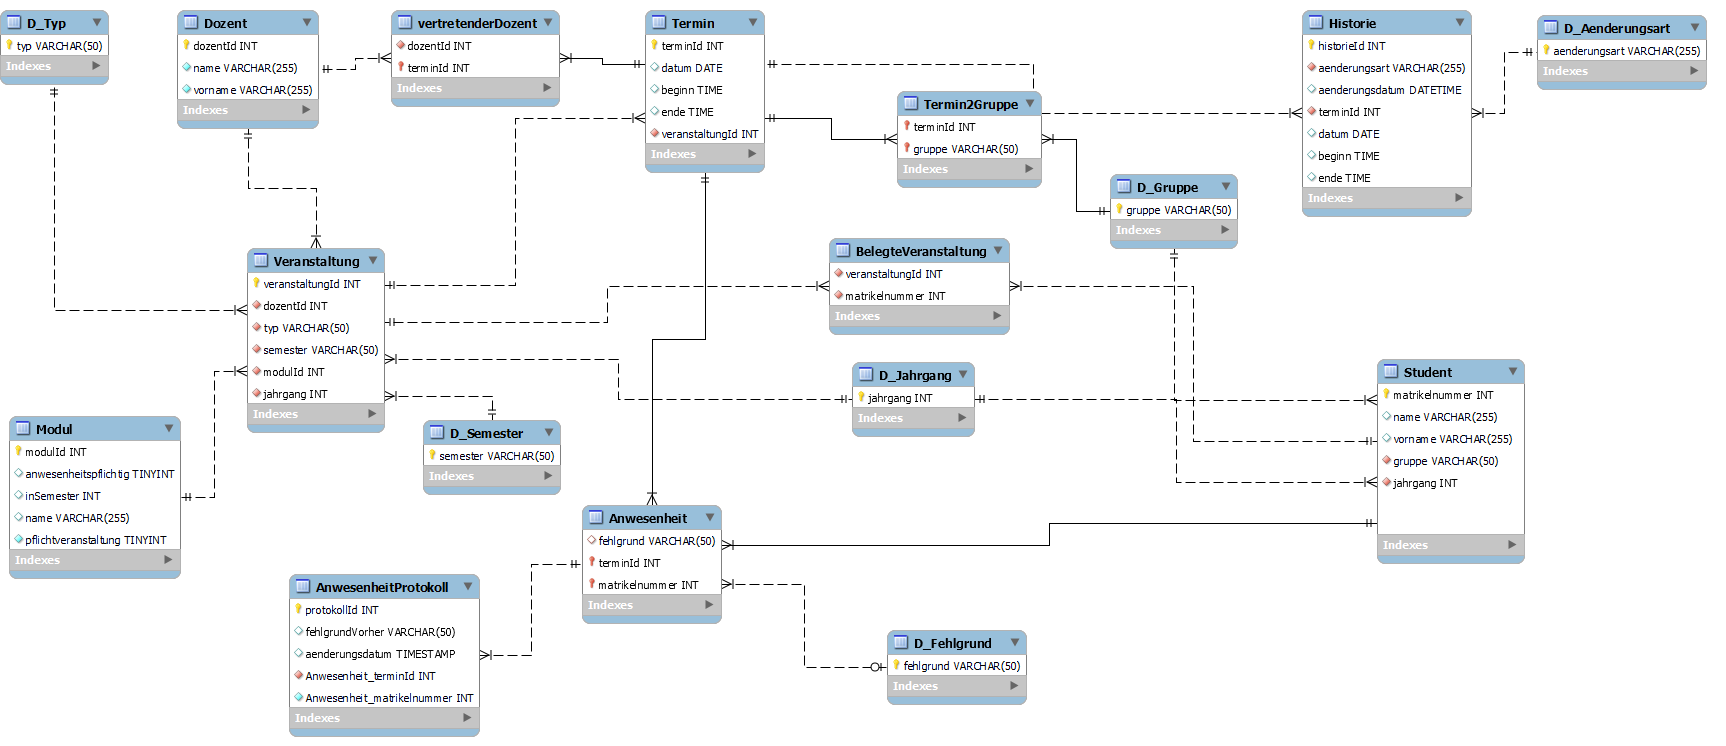
\includegraphics[width=\textwidth]{studenplanDBmodel.png}
Die Tabellen des jetzigen Datenbankschemas lassen sich in die drei Kategorien \textbf{Entity}, \textbf{Relation} und \textbf{Domain} unterteilen.

\vspace{12pt}

\subsubsection{Entity}
Eine Tabelle, die Fachliche Objekte bzw. Informationen Enthält, kann und wird in Neo4J durch Knoten dargestellt. Also wird jedes Tupel aus einer Entitäts-Tabelle zu einem Label. Die folgenden Tabellen wurden dieser Kategorie zugeteilt.
17
\begin{itemize}
	\item Dozent
	\item Termin
	\item Veranstaltung
	\item Modul
	\item Student
	\item Historie (Wird nicht weiter betrachtet, weil sich unserer Meinung nach neo4J schlecht dafür eignet eine Historie von Änderungen darzustellen)
\end{itemize}

\vspace{12pt}

\subsubsection{Releation}
Relationstabellen sind Matching Tabellen. Diese werden sich in Beziehungen zwischen den knoten auflösen. Die folgenden Tabellen wurden dieser Kategorie zugeteilt.

\begin{itemize}
	\item vertretenderDozent
	\item Termin2Gruppe (Wird nicht weiter mit einbezogen, weil diese Tabelle keine Rolle für Funktionsfähigkeit des Projektes spielt.)
	\item BelegteVeranstaltung
	\item Anwesenheit
\end{itemize}

\vspace{12pt}

\subsubsection{Domain}
Eine Domain Tabelle ist eine Tabelle, die in einer Relationalen Datenbank für die Konsistenz von Daten sorgt. So eine Tabelle besteht häufig nur aus einer Spalte. Dadurch soll sichergestellt werden, dass nur vordefinierte Werde benutzt werden können. Diese Tabellen werden beider Konvertierung zu Neo4J wegfallen. Die folgenden Tabellen wurden dieser Kategorie zugeteilt.

\begin{itemize}
	\item D\_Typ
	\item D\_Gruppe
	\item D\_Aenderungsart
	\item D\_Semester
	\item D\_Jahrgang
	\item D\_Fehlgrund	
\end{itemize}

\vspace{12pt}

\subsubsection{Ergebnis}
Wir haben die folgenden Labels und Beziehungen ausgearbeitet.

\vspace{6pt}

\paragraph{Labels}
\begin{itemize}
	\item Dozent
	\item Termin
	\item Modul
	\item Veranstaltung
	\item Student
\end{itemize}

\vspace{6pt}

\paragraph{Beziehungen}
\begin{itemize}
	\item VERTRITT\_IN
	\item BELEGT\_VERANSTALTUNG
	\item NICHT\_ANWESEND
	\item HAT
	\item LEITET
\end{itemize}

\newpage

\subsection{Erweiterungen}
Wir sollen drei sinnvolle Erweiterungen ausarbeiten. Einmal soll nachvollziehbar sein, welche Module aufeinander aufbauen. Zum anderen sollen Studenten, die das Modul gerade machen, Studenten finden können, die das Modul bereits abgeschlossen haben und um Hilfe bitten. 

\vspace{12pt}

\subsubsection{Aufeinander aufbauende Module}
Es gibt Module, die aufeinander aufbauen. Das wird im Jetzigen Zustand nicht von unserem Datenbankschema abgebildet. Es gibt bereits Modul-Knoten. Hier wird nur eine weitere Beziehung hinzugefügt, die \textbf{BASIERT\_AUF} heißt und darstellt, dass in dem Modul davon ausgegangen wird, dass andere Module bereits absolviert wurden.

\vspace{12pt}

\subsubsection{Vertiefungen}
Es gibt Vertiefungen. Eine Vertiefung ist eine Gruppierung von Modulen, die Logisch zusammen gehören und einzelne Themen eines Großen Themas behandeln. Im Augenblick gibt es keine Möglichkeit, die Gruppierung von Modulen darzustellen. Dafür muss ein neuer Knotentyp und eine neue Beziehung hinzugefügt werden. Der Knotentyp heißt \textbf{Vertiefung}. Die neue Beziehung heißt \textbf{BESTEHT\_AUS}. Eine Vertiefung hat einen Namen.

\vspace{12pt}

\subsubsection{Hilfe unter Studenten}
Zum anderen sollen Studenten, die das Modul gerade machen, Studenten finden können, die das Modul bereits abgeschlossen haben und um Hilfe bitten.

\newpage

\subsection{Daten}
Nachdem bestimmt wurde, wie die Daten gespeichert werden, sollen sinnvolle Daten gespeichert werden.

	
	\printnoidxglossaries
	
\end{document}